%!TEX root = ../vernier.tex
\subsection{Glyphs} \label{sec:glyphs}
The resulting dt-SNE projection is a set of points in 2D space, but we can still add a lot of information to the representation by means of color mapping, through glyphs size and shape, creating connection between points, and even by using the background's empty space to encode some other feature.

Figure \ref{fig:count_line} illustrates the initial tool set-up. Both the radius of the circular glyph and color are set to encode the number of lines of code metric. Right away we can start to identify cluster of points, indicating similarity on the $\mathbb{R}^{n}$ space, and outliers.

\begin{figure}[H]
  \centering
  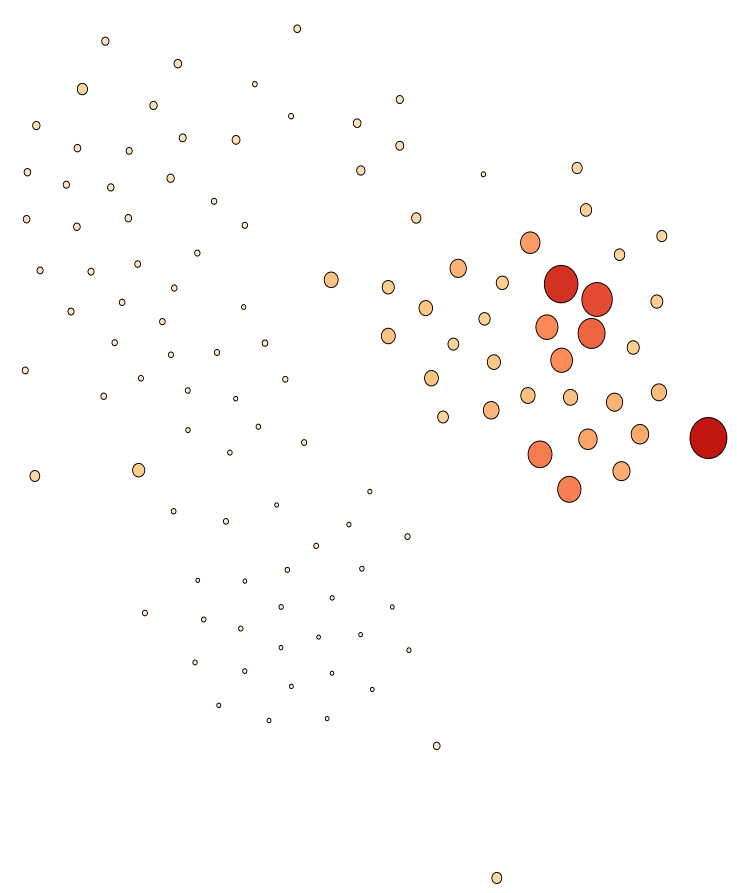
\includegraphics[width=0.7\textwidth]{figures/count_line.png}
  \caption{LOC metric displayed in both radius and color attributes}
  \label{fig:count_line}
\end{figure}

One example of use case is to change the color mapping to represent another metric. On figure \ref{fig:max_inh_tree}, the maximum inheritance tree depth metric for each class is coded in the glyph's color. This rich visualization allows us to reason about three different aspects of the data: entities's similarity (given by position), class size (given by the radius), and the number of intermediate classes between each data point and the root class of its inheritance tree (encoded in the color).

\begin{figure}[H]
  \centering
  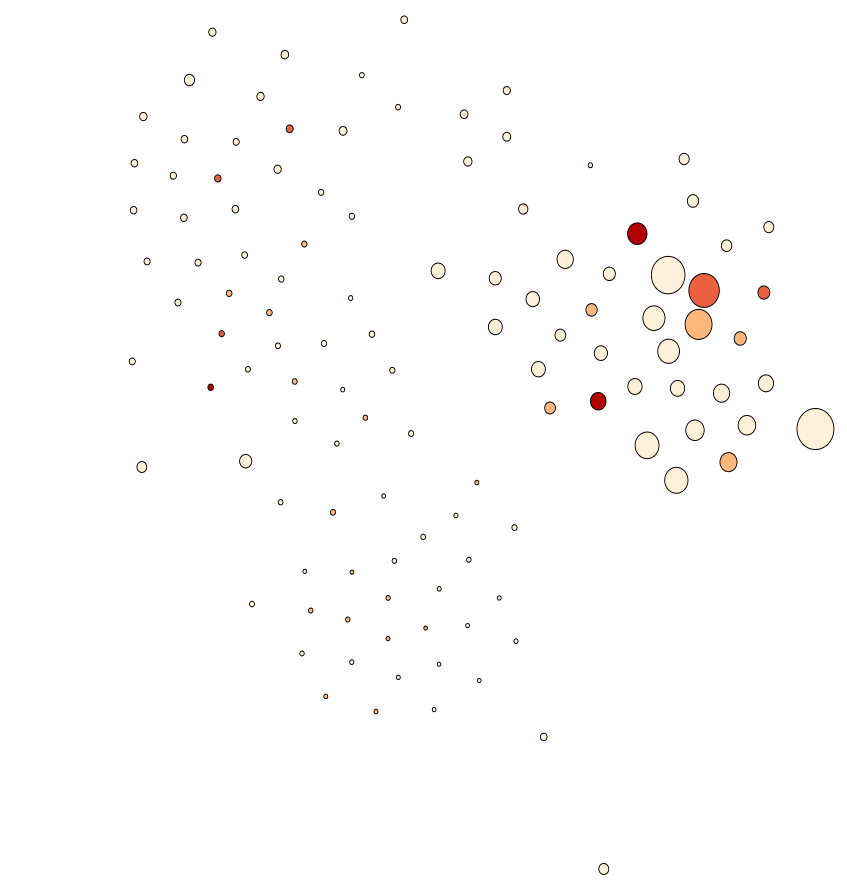
\includegraphics[width=0.6\textwidth]{figures/max_inh_tree.png}
  \caption{LOC metric displayed in both radius and color attributes}
  \label{fig:max_inh_tree}
\end{figure}

In order to add information about change of metric value to the projection, we have designed the glyph illustrated on figure \ref{fig:glyphs1}. The glyph's radius represents the normalized value of the metric in the current revision, and the angle of the pie section amounts to the percentual change in metric value from revision $T_{n-1}$ to $T_{n}$. If the metric increases in value, a pie section of larger radius is added to the top of the glyph, otherwise a pie section of smaller radius is placed on the bottom of the glyph representing the reduction percentage.

\begin{figure}[H]
  \centering
  
\includegraphics[width=0.3\textwidth]{figures/glyphs_1.png}
  \caption{Glyphs portraying 20\% increase and reduction on metric value}
  \label{fig:glyphs1}
\end{figure}

Although it's an interesting design, it has one major flaw: 80\% increase and 20\% decrease in value are represented by the same shape. This issue is fixed on the glyph shown on Figure \ref{fig:glyphs2}, where the decrease is portrayed by the removal of a pie section. In the application, the pie section is only drawn if the change in metric value is higher than $\pm1\%$, as shown in Figure \ref{fig:glyphs4}.

\begin{figure}[H]
  \centering
  
\includegraphics[width=0.3\textwidth]{figures/glyphs_2.png}
  \caption{Revised glyph}
  \label{fig:glyphs2}
\end{figure}

\begin{figure}[H]
  \centering
  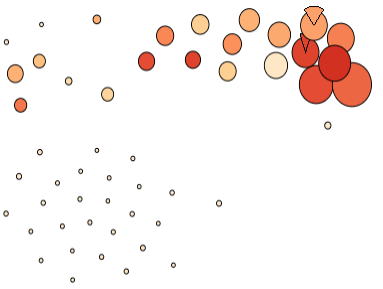
\includegraphics[width=0.5\textwidth]{figures/glyphs_4.png}
  \caption{Representation of 4 different aspects of the data.}
  \label{fig:glyphs4}
\end{figure}

What Figure \ref{fig:glyphs4} accomplishes is quite interesting. In a small space, we've encoded 4 different aspects of the data: similarity (position), class size (glyph radius), change in class size (delta pie slice size), and average cyclomatic complexity value for each class's methods (color). And best of all, without any clutter or misinformation.
